\subsection{Introduction}
\indent The unique requirements for the sensor developed for deployment on the Claiborn Pell Newport Bridge set the sensor apart from off-the-shelf sensors readily available for purchase.
The sensor package needed to record high precision, high resolution accelerometer and strain gauge data continuously for an extended period of time. 
The longevity of the package was dependent upon the battery capacity and data storage capacity. 
This could have been solved by utilizing a large bank of batteries and multiple hard disk drives; however it was determined that this was a not a feasible option. 
Instead the sensor package would scavenge energy to recharge batteries and transmit data to a base station wirelessly. 
The addition of these two requirements greatly increased the complexity of the sensor package design. \\

\indent 

\subsection{Circuitry}

\subsubsection{Voltage Regulation}
The voltage input for most systems on the sensor board are a range of voltages between 3.3V-5V.
This posed a basic issue due to the output voltage of the 12V battery. 
The solution was to use two LM317 linear voltage regulators.
It was initially proposed to use the two regulators in series, such that the voltage dropped from 12V to 5V and then to 3.3V.
However, due to the current rating on the devices, it was decided to use the regulators in parallel and drop the voltage from 12V to 5V and 12V to 3.3V.
The complete circuit may be found in Figure \ref{fig:Schematic_VoltageReg}.
The LM317 technical specifications are displayed in Table \ref{tab:LM317} 

\begin{table}[h]
\centering
\begin{tabular}{|l|c|}
\hline
\textbf{Parameter} & \textbf{Value}\\
\hline
Input Voltage Differential ($V_{in}-V_{out}$)& 3V $\le V_{in}-V_{out} \le$ 40V\\
Output Voltage ($V_{out}$) & 1.2V $\le V_{out} \le$ 37V\\
Output Current ($I_{out}$) & 1.5A\\
Max Power Dissipation ($P_{D}$) & 20W\\
Package Type				   & TO-220\\
\hline
\end{tabular}
\caption{LM317 Adjustable Linear Regulator Specifications}
\label{tab:LM317}
\end{table}

The output voltage can be set using Equation \ref{eqn:LM317} where $R_1= 240\Omega$ and $I_{adj}\le 100\mu A$.
It should be noted the $V$ is not the input voltage, but a unit placeholder.
Since $I_{adj}$ is very low, the error associated with it is almost negligible. 
\begin{equation}
V_{out} = 1.25V(1+\frac{R_2}{R_1}) + I_{adj}R_2
\label{eqn:LM317}
\end{equation}
The regulation circuit was tested using a 7.7Ah 12V battery in order to confirm the output voltages. %Possibly test and record range of input and output voltages
The voltages recorded were steady at approximately 3.5V and 5.3V.
The error is believed to be due to the inherent tolerance in the passive components used in the circuit.
Also in field use, the package will be subject to a wide range of temperatures that will cause the error in voltage to vary.

\subsubsection{ADC Impedance Matching}
\label{sec:ADC_Impedance_Matching}
As mentioned in Section \ref{sec:ADC_Impedance_Issues}, impedance matching issues were encountered when sampling accelerometer data with the micro-controller.
To avoid such issues in the final design, an impedance matching op-amp was used.
The MCP606 op-amp was used due to its rail-to-rail output, low input offset voltage, unity gain stability and low power characteristics. 
In order to act as a buffer for the input of the ADC, the op-amp was configured as in Figure \ref{fig:op-amp_standard}; where $R_1$ and $R_2$ are governed by the Equation \ref{eqn:op-amp_gain}. Since the op-amp will be used with unity gain (gain = 1) then both resistors are $0\Omega$ and essentially 

\begin{figure}
\centering
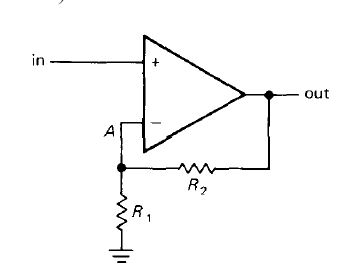
\includegraphics[scale=1]{Op-Amp_Standard}
\caption{Standard configuration of op-amp as a buffer}
\label{fig:op-amp_standard}
\end{figure}

\begin{equation}
gain = 1 + \frac{R_{2}}{R_{1}}
\label{eqn:op-amp_gain}
\end{equation}

\subsection{Printed Circuit Board}
\label{sec:PCB}